\chapter{I servizi del livello di collegamento e il framing}

\begin{center}
\begin{tikzpicture}[node distance=0pt]
  \node[lay app, minimum width=3.4cm] (a) {Applicazione};
  \node[lay tra, minimum width=3.4cm, below=of a] (t) {Trasporto};
  \node[lay net, minimum width=3.4cm, below=of t] (n) {Rete};
  \node[lay link, minimum width=3.4cm, below=of n, line width=1.5pt, draw=netred] (l) {\bfseries Collegamento};
  \node[lay phy, minimum width=3.4cm, below=of l, line width=1.5pt, draw=netred] (p) {\bfseries Fisico};
  \draw[-{Stealth}, thick, netred] ([xshift=0.3cm]l.south east) -- ++(1,0) node[right, lbl, text=netred] {siamo qui};
\end{tikzpicture}
\end{center}

% ══════════════════════════════════════════════════════════════
\section{Dalla rete al collegamento e al livello fisico}
% ══════════════════════════════════════════════════════════════

Ogni percorso che gli algoritmi di routing hanno calcolato è una sequenza di \textbf{singoli hop}, e non ci siamo mai chiesti che
cosa sia uno di essi. Sotto il livello di rete non c'è più nulla da instradare: ci sono due macchine unite da un canale, e dei bit
da far passare dall'una all'altra. Restano aperte due domande: \textbf{come sono impacchettati i bit} su quel canale, e \textbf{come
si chiama} la macchina all'altro capo. In questo capitolo e nel prossimo rispondiamo alla prima; il nome arriva con le reti locali,
dove più di due macchine condividono lo stesso filo e una di esse va indirizzata.

Il livello di rete fornisce comunicazione tra due host, \emph{ovunque} si trovino, e lo fa instradando. Il livello di
collegamento e il livello fisico forniscono invece comunicazione tra due nodi \textbf{direttamente collegati}: un tratto del
percorso, senza scelte da fare.

\begin{itemize}
    \item il \textbf{livello di collegamento} (\emph{link layer}) è la parte della pila dedicata alla trasmissione di pacchetti sui
          collegamenti (canali di trasmissione), \textbf{da un nodo al successivo} della rete;
    \item il \textbf{livello fisico} regola la struttura dei collegamenti (mezzo trasmissivo, connettori, tipi di cavo, \dots) e il modo
          in cui i bit vengono rappresentati e trasmessi lungo il collegamento.
\end{itemize}

\begin{figure}[H]
\centering
\begin{tikzpicture}[every node/.style={font=\scriptsize\sffamily}]
  \node[lay app, minimum width=2.2cm] at (0,2.4) {Applicazione};
  \node[lay tra, minimum width=2.2cm] at (0,1.8) {Trasporto};
  \node[lay net, minimum width=2.2cm] at (0,1.2) {Rete};
  \node[lay link, minimum width=2.2cm] at (0,0.6) {Collegamento};
  \node[lay phy, minimum width=2.2cm] at (0,0) {Fisico};
  \foreach \y/\t/\c in {2.1/{host -- host (processi)}/ltra, 1.2/{host -- host (instradamento)}/lnet, 0.3/{nodo -- nodo (un hop)}/llink} {
    \node[anchor=west, font=\footnotesize\sffamily] at (1.9,\y) {$\leftarrow$ \t};
  }
  \node[draw, fill=white, anchor=west, text width=6.8cm, align=left] at (6.2,1.2) {Collegamento e fisico sono strettamente intrecciati: spesso vengono raggruppati in un unico livello detto \textbf{network access} (o ``link + fisico''), e alcuni protocolli comuni, come Ethernet, coprono entrambi.};
\end{tikzpicture}
\caption{Cosa garantisce ciascun livello.}
\end{figure}

\dfn{Nodi e collegamenti}{
    \begin{itemize}
      \item Un \textbf{nodo} è qualsiasi dispositivo che esegue un protocollo di collegamento: host, router, switch, hub,
            access point Wi-Fi.
      \item Un \textbf{collegamento} (\emph{link}) è il canale di comunicazione che connette due nodi \textbf{adiacenti} lungo un
            percorso. Su di esso il nodo che trasmette incapsula il datagramma in un \textbf{frame} e lo mette sul canale.
    \end{itemize}
}

Nel grafo su cui abbiamo calcolato i percorsi un arco era un filo tra due router. Un collegamento non deve per forza essere
questo: può essere un \textbf{mezzo condiviso} da molti nodi contemporaneamente, e buona parte di ciò che fa questo livello esiste
proprio per questo.

Applicazione e trasporto vivono solo negli end system: uno switch non ha un livello di trasporto, un router non ha
un'applicazione. Collegamento e fisico, invece, sono presenti in \textbf{tutti} i pezzi dell'infrastruttura di rete:

\begin{itemize}
    \item \textbf{nodi}: host (PC, server, \dots), router, switch, hub, access point Wi-Fi;
    \item \textbf{collegamenti}: cablati (rame, fibra ottica) e senza fili (radiofrequenze).
\end{itemize}

Sono anche così intrecciati che spesso vengono raggruppati in un unico livello, \emph{network access}. Ethernet ne è il caso più
chiaro: un solo nome per un insieme di standard che specificano \textbf{sia il frame sia il segnale} sul filo.

\subsection{Un esempio di segnale: la codifica NRZ}

A questo livello non abbiamo altro che \textbf{bit} (zeri e uni) trasmessi su una linea fisica, rappresentati da grandezze fisiche.
L'esempio più semplice di codifica è la \textbf{NRZ} (\emph{Non-Return to Zero}): il tempo è diviso in intervalli uguali, e in ciascun
intervallo il segnale vale $+L$ per rappresentare un 1 e $0$ (oppure $-L$) per rappresentare uno 0.

\begin{figure}[H]
\centering
\begin{tikzpicture}[every node/.style={font=\footnotesize\sffamily}]
  \draw[-{Stealth}] (0,0) -- (8.6,0) node[right] {$t$};
  \draw[-{Stealth}] (0,-0.3) -- (0,1.6) node[above] {$s(t)$};
  \node[left] at (0,1) {$+L$}; \node[left] at (0,0) {0};
  \draw[very thick, netblue] (0,1) -- (1,1) -- (1,0) -- (2,0) -- (2,1) -- (4,1) -- (4,0) -- (6,0) -- (6,1) -- (7,1) -- (7,0) -- (8,0);
  \foreach \x/\b in {0.5/1, 1.5/0, 2.5/1, 3.5/1, 4.5/0, 5.5/0, 6.5/1, 7.5/0} \node at (\x,-0.35) {\b};
  \foreach \x in {1,...,8} \draw[dashed, black!30] (\x,0) -- (\x,1.3);
  \draw[netred, thick, decorate, decoration={brace, amplitude=4pt}] (2,1.15) -- (4,1.15) node[midway, above=5pt, text=netred, font=\scriptsize\sffamily] {due bit, un solo tratto piatto};
\end{tikzpicture}
\caption{La sequenza 10110010 in codifica NRZ: il tempo è diviso in intervalli uguali.}
\end{figure}

Due 1 consecutivi danno un \textbf{tratto piatto}: nessun fronte dice dove è finito il primo bit e dove è cominciato il secondo. Il
ricevente deve quindi sapere da sé dove cadono gli intervalli, e i due estremi devono essere d'accordo su quanto dura ciascuno.
Lasciando passare una lunga sequenza di bit uguali i due orologi \textbf{si allontanano} (\emph{clock drift}): è il motivo per cui le
codifiche usate davvero \textbf{forzano delle transizioni}, come vedremo parlando del livello fisico.

% ══════════════════════════════════════════════════════════════
\section{L'ultimo incapsulamento}
% ══════════════════════════════════════════════════════════════

Per consegnare un datagramma IP dall'host sorgente all'host destinazione bisogna farlo ``saltare'' su ciascuno dei singoli
collegamenti e dispositivi del percorso. Per essere trasferiti su un collegamento, i datagrammi vengono incapsulati in
\textbf{frame} di collegamento, il cui formato dipende dal tipo di collegamento.

\dfn{Frame}{
    Il livello di collegamento accetta pacchetti dal livello di rete e li incapsula in \textbf{frame}, che invia usando il livello
    fisico; in ricezione il processo è inverso. È l'\textbf{ultimo incapsulamento}: i frame vengono convertiti in \textbf{segnali} e
    trasferiti sul collegamento secondo le sue specifiche. I segnali possono essere impulsi elettrici, luce o onde radio.
}

\begin{figure}[H]
\centering
\begin{tikzpicture}[every node/.style={font=\scriptsize\sffamily}]
  \begin{scope}
    \node[font=\footnotesize\bfseries\sffamily] at (1.5,2.9) {Mittente};
    \node[lay net, minimum width=3cm] (n1) at (1.5,2.2) {rete};
    \node[lay link, minimum width=3cm] (l1) at (1.5,1.1) {collegamento};
    \node[lay phy, minimum width=3cm] (p1) at (1.5,0) {fisico};
    \node[field, fill=lnet!70, minimum width=1.4cm] at (1.5,2.2) {pacchetto};
    \node[field, fill=llink, minimum width=0.4cm] (h) at (0.65,1.1) {H};
    \node[field, fill=lnet!70, minimum width=1.4cm, right=0pt of h] (pl) {payload};
    \node[field, fill=llink, minimum width=0.4cm, right=0pt of pl] {T};
  \end{scope}
  \begin{scope}[xshift=8cm]
    \node[font=\footnotesize\bfseries\sffamily] at (1.5,2.9) {Ricevente};
    \node[lay net, minimum width=3cm] (n2) at (1.5,2.2) {rete};
    \node[lay link, minimum width=3cm] (l2) at (1.5,1.1) {collegamento};
    \node[lay phy, minimum width=3cm] (p2) at (1.5,0) {fisico};
  \end{scope}
  \draw[dashed, thick, netblue, {Stealth}-{Stealth}] (l1.east) -- node[above] {percorso virtuale dei dati (frame)} (l2.west);
  \draw[very thick, netred, {Stealth}-{Stealth}] (p1.east) -- node[below] {percorso reale: segnali sul mezzo} (p2.west);
  \draw[-{Stealth}, thick] (n1) -- (l1); \draw[-{Stealth}, thick] (l1) -- (p1);
  \draw[-{Stealth}, thick] (p2) -- (l2); \draw[-{Stealth}, thick] (l2) -- (n2);
\end{tikzpicture}
\caption{Il frame: header (H), payload (il pacchetto di rete) e trailer (T).}
\end{figure}

\begin{itemize}
    \item Header, payload, trailer: è la prima volta che un livello mette qualcosa \textbf{dopo} i dati, perché il controllo che sta nel
          trailer copre tutto ciò che lo precede.
    \item Il payload più grande che un frame può portare è la \textbf{MTU}: il numero che decideva dove un datagramma andava
          frammentato.
    \item È comodo pensare a due livelli di collegamento che si parlano; i bit, in realtà, scendono, attraversano il mezzo e
          risalgono.
\end{itemize}

\subsection{Sei collegamenti tra un portatile e un server}

Seguiamo un datagramma da un portatile collegato in Wi-Fi fino a un server all'altro capo di una piccola rete: Wi-Fi fino
all'access point, Ethernet fino allo switch, dallo switch al router, da router a router, poi giù fino all'altro switch e al server.

\begin{figure}[H]
\centering
\begin{tikzpicture}[every node/.style={font=\scriptsize\sffamily}]
  \node (n1) at (0,0) {\icon[0.85cm]{laptop}};
  \node (n2) at (2.2,0) {\icon[0.75cm]{accesspoint}};
  \node (n3) at (4.4,0) {\icon[0.9cm]{switch}};
  \node (n4) at (6.6,0) {\icon[0.8cm]{router}};
  \node (n5) at (8.8,0) {\icon[0.8cm]{router}};
  \node (n6) at (11,0) {\icon[0.9cm]{switch}};
  \node (n7) at (13.2,0) {\icon[0.45cm]{server}};
  \foreach \n/\t in {n1/portatile, n2/access point, n3/switch, n4/router, n5/router, n6/switch, n7/server}
    \node[below=-1pt of \n] {\t};
  \draw[thick, netorange, decorate, decoration={snake, amplitude=1.2pt, segment length=5pt}] (n1) -- node[above=5pt] {1: Wi-Fi} (n2);
  \draw[wired] (n2) -- node[above=3pt] {2: Ethernet} (n3);
  \draw[wired] (n3) -- node[above=3pt] {3: Ethernet} (n4);
  \draw[line width=1.1pt, netgreen!60!black] (n4) -- node[above=3pt] {4: fibra} (n5);
  \draw[wired] (n5) -- node[above=3pt] {5: Ethernet} (n6);
  \draw[wired] (n6) -- node[above=3pt] {6: Ethernet} (n7);
  \node[field, fill=lnet!60, minimum width=1.3cm] (dg) at (6.6,-1.45) {datagramma};
  \node[font=\scriptsize\sffamily] at (6.6,-2.1) {lo stesso datagramma attraversa tutti e sei i collegamenti; il frame che lo avvolge è costruito e buttato via a ogni hop};
\end{tikzpicture}
\caption{Sei collegamenti, ciascuno con il suo frame: radio, doppino e fibra, ognuno con il proprio protocollo.}
\end{figure}

Ognuno dei sei collegamenti porta il datagramma dentro un \textbf{frame suo}, costruito e buttato via su quell'hop. I collegamenti
non si somigliano: radio qui, doppino là, fibra nel mezzo, ciascuno con il suo protocollo.

\begin{itemize}
    \item A ogni nodo il frame viene aperto, il datagramma estratto e \textbf{reimpacchettato} in un frame di tipo diverso.
    \item Anche i \textbf{servizi} cambiano: un collegamento può riscontrare ogni frame, quello successivo può scartare frame senza
          dire nulla.
    \item Per questo i livelli superiori non possono contarci: IP è progettato per funzionare \textbf{su qualunque cosa ci sia sotto},
          ed è il motivo per cui le garanzie vengono ricostruite \textbf{da un estremo all'altro}.
    \item Ciò che attraversa il percorso invariato è il \textbf{datagramma} (a parte i due campi che ogni router riscrive, TTL e
          checksum dell'header); ciò che cambia a ogni passo è l'\textbf{involucro}.
\end{itemize}

% ══════════════════════════════════════════════════════════════
\section{I servizi del livello di collegamento}
% ══════════════════════════════════════════════════════════════

Un protocollo di collegamento può offrire fino a \textbf{quattro servizi}. Quali offrire è una scelta di progetto, e collegamenti
diversi scelgono in modo diverso: solo il primo è offerto praticamente da tutti, gli altri tre sono facoltativi, e le ragioni
meritano di essere capite.

\subsection{1. Framing}

Incapsulare i datagrammi in frame, con il datagramma come payload e un header e un trailer specifici. La struttura del frame dipende
dai protocolli di collegamento e fisico.

\subsection{2. Accesso al collegamento (link access)}

Definire le regole di accesso al collegamento tramite un protocollo \textbf{MAC} (\emph{Medium Access Control}). Le regole
dipendono dall'architettura del collegamento:

\begin{itemize}
    \item nei collegamenti \textbf{punto-punto} (un solo mittente e un solo ricevente) il protocollo MAC è semplice o inesistente:
          il mittente può inviare un frame ogni volta che il collegamento è libero;
    \item nei collegamenti \textbf{broadcast} molti nodi stanno sullo stesso mezzo, e ciò che uno trasmette è sentito da tutti: due
          che trasmettono insieme si distruggono a vicenda il frame. È il \textbf{problema dell'accesso multiplo}, e il protocollo MAC
          serve a coordinare chi trasmette e quando.
\end{itemize}

Il MAC è un \textbf{sottolivello} del livello di collegamento: sopra di esso stanno framing e controllo degli errori, sotto il
livello fisico. È la parte che decide \textbf{quando} si può trasmettere, ed è l'argomento del capitolo sull'accesso multiplo.

\warning{Attenzione alla parola}{
    Qui \emph{broadcast} descrive la \textbf{natura del canale} (tutti sentono tutto), non l'invio di un messaggio a tutti i
    destinatari come per l'indirizzo di broadcast IP.
}

\subsection{3. Consegna affidabile}

Garantire che un frame consegnato a questo collegamento arrivi all'altro capo. Le garanzie sono le tre che abbiamo già smontato
al livello di trasporto (niente perso, niente duplicato, tutto in ordine), ricostruite \textbf{un hop alla volta}, e il macchinario è
lo stesso: riscontri, timer, numeri di sequenza, ritrasmissioni. Cambia solo la distanza.

\begin{itemize}
    \item \textbf{Dove conviene}: sui collegamenti che perdono spesso, come quelli \textbf{senza fili}. L'errore viene riparato
          \textbf{dove è avvenuto}, in una frazione di round trip, senza costringere gli estremi a ritrasmettere.
    \item \textbf{Dove non conviene}: su fibra, coassiale e doppino il tasso di errore è così basso che i riscontri costano più delle
          perdite. Per questo molti protocolli cablati, Ethernet compreso, semplicemente \textbf{non la offrono}.
\end{itemize}

\begin{table}[H]
\centering
\begin{tabular}{lccl}
\toprule
\textbf{Servizio} & \textbf{Riscontri} & \textbf{Connessione} & \textbf{Esempio} \\
\midrule
Senza riscontro, senza connessione & no & no & Ethernet \\
Con riscontro, senza connessione & sì & no & 802.11 (Wi-Fi) \\
Con riscontro, orientato alla connessione & sì & sì & lunghi collegamenti satellitari \\
\bottomrule
\end{tabular}
\caption{Le tre classi di servizio di un collegamento.}
\end{table}

\begin{itemize}
    \item La prima va bene quando gli errori sono rari, e anche per voce e video, dove un dato in ritardo è peggio di un dato
          sbagliato.
    \item La seconda ritrasmette un frame che non è stato riscontrato in tempo: è ciò che serve a un collegamento senza fili, e
          non a una fibra.
    \item La terza numera ogni frame e garantisce che ciascuno arrivi \textbf{esattamente una volta e in ordine}: un flusso di bit
          affidabile, costruito su un solo hop.
\end{itemize}

\info{Riscontrare qui è un'ottimizzazione}{
    Non è mai un requisito: i due estremi possono sempre inviare, aspettare e ripetere tutto quando non torna nulla. Il problema è
    l'\textbf{efficienza}. Un collegamento ha una dimensione massima del frame, quindi un pacchetto grande parte come, diciamo,
    \textbf{dieci frame}: se due si perdono e nessuno se ne occupa sul collegamento, toccherà rimandarli \textbf{tutti e dieci},
    da un estremo all'altro e secondi dopo. Il collegamento conosce la propria dimensione di frame, il proprio ritardo e il proprio
    tasso d'errore, che i livelli superiori non conoscono: può riparare a poco prezzo. E non toglie nulla ai livelli sopra:
    un'ottimizzazione su un hop \textbf{non è una garanzia} su un percorso.
}

\subsection{4. Rilevazione e correzione degli errori}

L'hardware di collegamento può subire il problema dell'\textbf{inversione dei bit} (\emph{bit flipping}): per attenuazione e
rumore elettromagnetico, l'hardware che riceve legge un 1 dove era stato inviato uno 0. Molti protocolli di collegamento
implementano strategie di controllo e correzione più sofisticate (e realizzate in hardware), in aggiunta a quelle dei livelli
superiori (i checksum di TCP e IP).

\begin{itemize}
    \item Non ha senso portare più avanti un datagramma danneggiato: il controllo si fa \textbf{a ogni hop}, dall'hardware che ha
          ricevuto il frame.
    \item Poiché non c'è un ulteriore incapsulamento, questi controlli coprono \textbf{l'intero frame}, header compresi.
    \item Essendo in hardware, possono permettersi di essere molto più accurati della somma a 16 bit che il trasporto calcola in
          software.
    \item \textbf{Rilevazione} e \textbf{correzione} sono due cose diverse: la prima dice che un frame è sbagliato, la seconda dice
          quali bit lo sono e li ripara. Il come è l'argomento del prossimo capitolo.
\end{itemize}

\subsection{E il controllo di flusso?}

Un mittente veloce e un ricevente lento: anche senza alcun errore, i frame arrivano più in fretta di quanto possano essere
assorbiti, e qualcuno si perde. Le soluzioni possibili sono due:

\begin{itemize}
    \item \textbf{basata su feedback}: il ricevente dice al mittente quando può inviare ancora, la stessa forma della finestra vista
          al livello di trasporto, su un solo hop;
    \item \textbf{basata sul tasso}: il protocollo limita la velocità di invio senza alcun feedback. Appartiene al livello di
          trasporto, non a questo.
\end{itemize}

Sul collegamento il controllo di flusso è quasi scomparso: l'hardware è costruito per lavorare \textbf{alla velocità del filo}
(\emph{wire speed}) e gestisce i frame alla stessa velocità con cui il collegamento li consegna. Un sovraccarico, a quel punto, non
è colpa del collegamento, e occuparsene è compito dei livelli superiori.

% ══════════════════════════════════════════════════════════════
\section{L'implementazione: la NIC}
% ══════════════════════════════════════════════════════════════

Nei dispositivi di rete (end system, router, \dots) le funzioni del livello di collegamento sono realizzate sia in software sia,
soprattutto, in hardware: gran parte di questo livello \textbf{non è software}, ma sta su un chip.

\begin{figure}[H]
\centering
\begin{minipage}{0.45\linewidth}\centering
  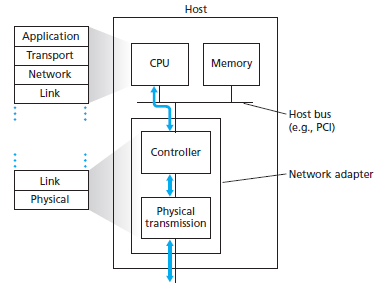
\includegraphics[width=0.85\linewidth]{cap18/nic_schema.png}
\end{minipage}\hfill
\begin{minipage}{0.45\linewidth}\centering
  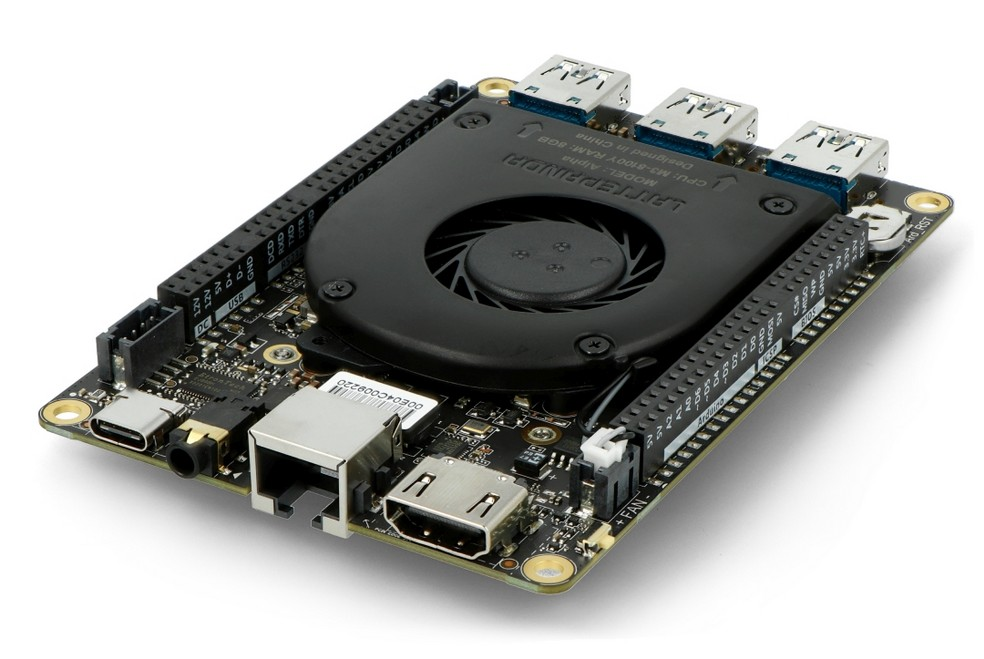
\includegraphics[width=0.85\linewidth]{cap18/nic.png}
\end{minipage}
\caption{A sinistra lo schema di un adattatore di rete collegato al bus dell'host; a destra un mini-PC (LattePanda) con la NIC integrata sulla scheda madre.}
\end{figure}

Nei computer ci sono adattatori di rete detti \textbf{NIC} (\emph{Network Interface Card}), con un chip specializzato
(\textbf{controller}) che realizza le funzioni di collegamento.

\begin{itemize}
    \item \textbf{In uscita} il controller prende il datagramma dalla memoria dell'host, lo incapsula in un frame, calcola i bit di
          rilevazione degli errori e trasmette.
    \item \textbf{In ingresso} riceve l'intero frame, lo controlla e passa il datagramma al livello superiore.
    \item Le due metà si incontrano sul \textbf{bus dell'host}: sotto l'adattatore, sopra CPU e memoria.
\end{itemize}

Un tempo gli adattatori erano schede separate dalla scheda madre (inserite negli slot PCI); oggi la funzione sta nel chipset
della scheda madre (\emph{LAN-on-motherboard}) o in un singolo chip dedicato ed economico. È cambiato l'imballaggio, non la
stratificazione: c'è ancora un controller, e fa ancora lo stesso lavoro.

\subsection{Software e hardware}

\begin{itemize}
    \item \textbf{Software}: gira sulla CPU e offre funzioni di alto livello come l'indirizzamento, la gestione di interrupt e
          hardware, la gestione degli errori, l'incapsulamento e il decapsulamento dei datagrammi.
    \begin{itemize}
      \item A livello di collegamento c'è un indirizzo aggiuntivo, l'\textbf{indirizzo MAC}, che identifica la NIC.
      \item I datagrammi vanno letti dalla memoria in incapsulamento (lato mittente) e scritti in memoria in decapsulamento (lato
            ricevente), perché li usi il protocollo superiore.
    \end{itemize}
    \item \textbf{Hardware}, sul controller: framing, controllo degli errori, regole di accesso al mezzo e conversione dei bit nel
          segnale da trasmettere secondo il protocollo fisico (Ethernet, wireless, \dots). Funziona come un tipico dispositivo di I/O.
\end{itemize}

Questa divisione è il motivo per cui il livello è veloce: ciò che va fatto \textbf{per ogni bit} non tocca mai il processore. Ed è
esattamente il lavoro che la porta d'ingresso di un router svolge su ciascuna delle sue interfacce: \textbf{terminare il
collegamento}.

\subsection{Le tecnologie fisiche}

Il protocollo di collegamento, e quindi la struttura del frame, dipende dalla tecnologia del collegamento fisico:

\begin{itemize}
    \item \textbf{Ethernet 802.3}: collegamento cablato basato su impulsi elettrici su cavi in rame con 4 doppini intrecciati (il più
          comune) o su fotoni in cavi di fibra ottica;
    \item \textbf{Wi-Fi 802.11}: collegamento senza fili a radiofrequenza (2,4 GHz, 5 GHz, 6 GHz);
    \item \textbf{Bluetooth}: collegamento senza fili a radiofrequenza (2,4 GHz), su brevi distanze.
\end{itemize}

Non c'è quindi un unico formato di frame da imparare: ce n'è \textbf{uno per tecnologia}, e ciò che hanno in comune è il compito,
non la disposizione dei campi. Pro e contro dei mezzi fisici (radio, doppino, fibra) sono confrontati nel capitolo sul livello
fisico.

% ══════════════════════════════════════════════════════════════
\section{I metodi di framing}
% ══════════════════════════════════════════════════════════════

Che cosa consegna il livello fisico al livello di collegamento? Un \textbf{flusso grezzo di bit}, e nient'altro: nessun segno,
nessun separatore, niente che dica dove qualcosa comincia o finisce.

\begin{itemize}
    \item Non è nemmeno garantito corretto: alcuni bit possono aver cambiato valore, e il \textbf{numero} di bit ricevuti può perfino
          essere diverso da quello inviato.
    \item Dove il canale è rumoroso il livello fisico aggiunge ridondanza ai propri segnali, ma questo \textbf{abbassa} il tasso di
          errore, non lo elimina.
    \item Tutto il resto va ricostruito da quella sequenza di zeri e uni, dal livello che le sta sopra.
\end{itemize}

Potremmo allora trasmettere un flusso ininterrotto di bit? No: senza confini non ci sarebbe nulla \textbf{in cui trovare un errore},
e nulla da \textbf{ritrasmettere} se non tutto. Inoltre i diversi pacchetti consegnati dal livello di rete arriverebbero come un'unica
sequenza indistinguibile. Per questo il flusso viene tagliato in \textbf{frame}: pezzi limitati, ciascuno con un inizio, una fine e
un controllo proprio. È l'unico servizio di cui nessun protocollo di collegamento può fare a meno, e quello che rende possibili gli
altri.

\dfn{Che cosa deve ottenere il framing}{
    I confini non sono nei bit: sono una struttura imposta su un flusso continuo, e il ricevente li deve trovare.
    \begin{itemize}
      \item \textbf{Facili da trovare}: il ricevente deve individuare l'inizio di un frame senza fatica, e i marcatori devono costare
            poco in termini di canale.
      \item \textbf{Recuperabili}: dopo un errore il ricevente deve potersi \textbf{risincronizzare}, cioè trovare dove inizia il
            frame successivo senza sapere nulla di quello andato male.
    \end{itemize}
    È il secondo requisito a separare i metodi, ed è quello che un primo tentativo sbaglia sempre.
}

I metodi principali sono quattro:

\begin{enumerate}
    \item conteggio dei byte (\emph{byte count});
    \item byte di flag con \emph{byte stuffing};
    \item bit di flag con \emph{bit stuffing};
    \item violazioni della codifica fisica.
\end{enumerate}

I primi tre lavorano \textbf{dentro} il flusso di bit, e devono quindi fare i conti con dati che imitano i marcatori. Il quarto prende
in prestito dal livello fisico un segnale che i dati \textbf{non possono produrre} affatto.

\subsection{Conteggio dei byte}

\dfn{Byte count}{
    Ogni frame inizia con un campo che indica il \textbf{numero di byte} del frame. È semplice, ma è difficilissimo
    risincronizzarsi dopo un errore, e in pratica non è mai usato da solo.
}

\begin{figure}[H]
\centering
\begin{tikzpicture}[every node/.style={font=\scriptsize\ttfamily}, b/.style={draw, minimum size=0.45cm, inner sep=0pt}]
  \node[font=\footnotesize\bfseries\sffamily, anchor=west] at (-0.5,0.7) {Senza errori};
  \foreach \v/\c [count=\i] in {5/netred!30,1/white,2/white,3/white,4/white, 5/netred!30,6/white,7/white,8/white,9/white, 8/netred!30,0/white,1/white,2/white,3/white,4/white,5/white,6/white, 8/netred!30,7/white,8/white,9/white,0/white,1/white,2/white,3/white}
     \node[b, fill=\c] at (\i*0.45,0) {\v};
  \draw[decorate, decoration={brace, amplitude=4pt, mirror}] (0.25,-0.35) -- (2.4,-0.35) node[midway, below=4pt, font=\scriptsize\sffamily] {frame 1: 5 byte};
  \draw[decorate, decoration={brace, amplitude=4pt, mirror}] (2.5,-0.35) -- (4.65,-0.35) node[midway, below=4pt, font=\scriptsize\sffamily] {frame 2: 5 byte};
  \draw[decorate, decoration={brace, amplitude=4pt, mirror}] (4.75,-0.35) -- (8.25,-0.35) node[midway, below=4pt, font=\scriptsize\sffamily] {frame 3: 8 byte};
  \draw[decorate, decoration={brace, amplitude=4pt, mirror}] (8.35,-0.35) -- (11.85,-0.35) node[midway, below=4pt, font=\scriptsize\sffamily] {frame 4: 8 byte};
  \begin{scope}[yshift=-2cm]
    \node[font=\footnotesize\bfseries\sffamily, anchor=west] at (-0.5,0.7) {Con un errore};
    \foreach \v/\c [count=\i] in {5/netred!30,1/white,2/white,3/white,4/white, 7/netorange!60,6/white,7/white,8/white,9/white, 8/white,0/white,1/white,2/white,3/white,4/white,5/white,6/white, 8/white,7/white,8/white,9/white,0/white,1/white,2/white,3/white}
       \node[b, fill=\c] at (\i*0.45,0) {\v};
    \draw[-{Stealth}, netorange, thick] (2.7,0.9) -- (2.7,0.3); \node[font=\scriptsize\sffamily, text=netorange] at (2.7,1.1) {errore: 5 diventa 7};
    \draw[decorate, decoration={brace, amplitude=4pt, mirror}] (2.5,-0.35) -- (5.55,-0.35) node[midway, below=4pt, font=\scriptsize\sffamily, text=netred] {frame 2 (sbagliato)};
    \draw[-{Stealth}, netred, thick] (5.85,-1.1) -- (5.85,-0.3); \node[font=\scriptsize\sffamily, text=netred, anchor=west] at (6,-1.0) {ora questo viene letto come un conteggio};
  \end{scope}
\end{tikzpicture}
\caption{Con il conteggio dei byte un solo errore sul contatore fa perdere la sincronizzazione su tutti i frame successivi.}
\end{figure}

Nella riga in basso un solo bit invertito ha trasformato un conteggio di 5 in 7, e il ricevente prende un byte di dati per il
conteggio successivo. Il controllo degli errori dirà che il frame è sbagliato, ma \textbf{non dove inizia il prossimo}, e nemmeno una
ritrasmissione aiuta: il ricevente ha perso il filo per sempre.

\subsection{Byte di flag e byte stuffing}

\dfn{Byte stuffing}{
    Ogni frame è delimitato da uno speciale \textbf{byte di flag} (FLAG). Se il byte FLAG compare \textbf{nei dati}, va
    ``protetto'' inserendo prima di esso un byte di escape (ESC); lo stesso vale per un ESC che compare nei dati. Il ricevente
    rimuove ogni ESC e considera come dato il byte che lo segue.
}

\begin{figure}[H]
\centering
\begin{tikzpicture}[every node/.style={font=\scriptsize\sffamily}, b/.style={draw, minimum height=0.45cm, minimum width=0.75cm, inner sep=1pt}]
  \node[b, fill=netred!25] (f1) at (0,0) {FLAG}; \node[b, right=0pt of f1, minimum width=1.2cm] (hd) {header};
  \node[b, right=0pt of hd, minimum width=4cm] (pl) {payload}; \node[b, right=0pt of pl, minimum width=1.2cm] (tr) {trailer};
  \node[b, fill=netred!25, right=0pt of tr] {FLAG};
  \node[font=\footnotesize\sffamily\bfseries, anchor=east] at (-0.6,0) {formato del frame};
  \node[font=\footnotesize\bfseries\sffamily] at (2,-0.8) {dati originali}; \node[font=\footnotesize\bfseries\sffamily] at (7.2,-0.8) {dopo lo stuffing};
  \tikzset{bw/.style={b, fill=white}, by/.style={b, fill=llink!70}, bs/.style={b, fill=netred!20}}
  \foreach \row/\orig/\stuf in {
     0/{A/bw,FLAG/by,B/bw}/{A/bw,ESC/bs,FLAG/by,B/bw},
     1/{A/bw,ESC/by,B/bw}/{A/bw,ESC/bs,ESC/by,B/bw},
     2/{A/bw,ESC/by,FLAG/by,B/bw}/{A/bw,ESC/bs,ESC/by,ESC/bs,FLAG/by,B/bw},
     3/{A/bw,ESC/by,ESC/by,B/bw}/{A/bw,ESC/bs,ESC/by,ESC/bs,ESC/by,B/bw}} {
    \foreach \x/\st [count=\i] in \orig \node[\st] at (0.8+\i*0.75,-1.4-\row*0.65) {\x};
    \draw[-{Stealth}, thick] (4.2,-1.4-\row*0.65) -- (4.9,-1.4-\row*0.65);
    \foreach \x/\st [count=\i] in \stuf \node[\st] at (4.9+\i*0.75,-1.4-\row*0.65) {\x};
  }
\end{tikzpicture}
\caption{Byte stuffing: ogni FLAG o ESC nei dati viene preceduto da un ESC.}
\end{figure}

\begin{itemize}
    \item Il FLAG marca \textbf{entrambi gli estremi} del frame: due FLAG di seguito sono la fine di un frame e l'inizio del
          successivo.
    \item Il frame diventa \textbf{più lungo}, ma dopo un errore è \textbf{facile risincronizzarsi}: basta cercare due FLAG. Si perde
          un frame, non il resto del flusso.
    \item Lo stuffing non è un'eventualità remota: con una foto o una canzone nel payload il byte FLAG comparirà \textbf{di sicuro}. È
          il metodo usato da \textbf{PPP}.
\end{itemize}

\subsubsection*{Il destuffing in ricezione}

La regola è meccanica e non richiede interpretazione: si \textbf{scarta il primo ESC} di una coppia e si prende \textbf{alla lettera}
il byte che lo segue, qualunque esso sia. Così ESC-FLAG diventa un FLAG di dati, ESC-ESC un ESC di dati.

\begin{itemize}
    \item Ciò che viene consegnato al livello superiore è \textbf{esattamente} ciò che era stato consegnato in trasmissione: il livello
          sopra non viene mai a sapere che qualcosa è stato inserito.
    \item I confini dei frame si trovano anche senza disfare gli escape: un FLAG preceduto da ESC è un dato, un FLAG non preceduto da
          ESC è un confine.
\end{itemize}

\subsection{Bit di flag e bit stuffing}

\dfn{Bit stuffing}{
    Il flag che delimita i frame è la sequenza di bit \texttt{01111110} (sei 1 consecutivi). Per evitare che compaia nei dati:
    \begin{itemize}
      \item \textbf{in trasmissione}, dopo \textbf{cinque 1 consecutivi} nei dati si inserisce uno \textbf{0};
      \item \textbf{in ricezione}, ogni \textbf{0 che segue cinque 1} viene eliminato.
    \end{itemize}
}

\begin{figure}[H]
\centering
\begin{tikzpicture}[every node/.style={font=\small\ttfamily}]
  \node[anchor=east, font=\footnotesize\sffamily] at (-0.2,0) {dati};
  \node[anchor=west] at (0,0) {0110111111111111111110010};
  \node[anchor=east, font=\footnotesize\sffamily] at (-0.2,-0.8) {trasmessi};
  \node[anchor=west] at (0,-0.8) {011011111\textcolor{netred}{\textbf{0}}11111\textcolor{netred}{\textbf{0}}11111\textcolor{netred}{\textbf{0}}10010};
  \node[anchor=east, font=\footnotesize\sffamily] at (-0.2,-1.6) {ricevuti};
  \node[anchor=west] at (0,-1.6) {0110111111111111111110010};
  \node[font=\footnotesize\sffamily, text=netred, anchor=west] at (7.2,-0.8) {bit di stuffing inseriti};
\end{tikzpicture}
\caption{Bit stuffing: dopo cinque 1 si aggiunge uno 0, che il ricevente rimuove.}
\end{figure}

\begin{itemize}
    \item Sei 1 consecutivi \textbf{non possono mai comparire} dentro un frame: un ricevente che ha perso la sincronizzazione deve solo
          cercare il flag.
    \item Il metodo non è legato ai byte (un frame può avere un numero qualsiasi di bit) e garantisce che sulla linea ci siano
          \textbf{transizioni}: per questo lo usa anche \textbf{USB}.
\end{itemize}

\subsection{Quanto costa lo stuffing}

E se il payload fosse fatto \textbf{solo di byte FLAG}? Con il byte stuffing ognuno di essi viene preceduto da un ESC: cento byte di
dati partono come circa \textbf{duecento}. Il frame è raddoppiato, e nessuno sopra l'aveva chiesto.

\begin{itemize}
    \item Con il bit stuffing il caso peggiore è più mite: ogni byte \texttt{01111110} si prende un solo bit in più, circa
          \textbf{un ottavo}; anche con un payload di soli 1 si aggiunge un bit ogni cinque. Ma la proprietà è la stessa.
    \item La proprietà: la \textbf{lunghezza del frame dipende da ciò che contiene}, e né il mittente né il ricevente possono prevederla
          dalla sola dimensione del payload.
\end{itemize}

È una delle ragioni per volere un delimitatore che i dati \textbf{non possano imitare} affatto.

\subsection{Violazioni della codifica fisica}

Si sfrutta la codifica della trasmissione fisica. Le codifiche fisiche spendono di solito \textbf{più simboli di quanti ne
servano ai dati}, proprio per forzare le transizioni di cui vive il ricevente.

\begin{itemize}
    \item Nella codifica \textbf{4B/5B} quattro bit di dati sono inviati come cinque bit di segnale: dei 32 simboli possibili, 16
          \textbf{non sono mai prodotti} dai dati.
    \item Se ne riservano due per significare \emph{inizio frame} e \emph{fine frame}: sono \textbf{violazioni della codifica},
          segnali che il payload non può imitare perché non ha modo di chiederli.
    \item \textbf{Il guadagno}: niente stuffing, niente che cresca, e un confine inconfondibile, perché il delimitatore sta
          \textbf{fuori dall'alfabeto} che i dati possono usare.
    \item \textbf{Il prezzo}: il metodo appartiene a \textbf{una} codifica fisica. Cambiata la codifica sottostante, i delimitatori
          spariscono.
\end{itemize}

\subsection{In pratica i metodi si combinano}

\begin{itemize}
    \item Ethernet e 802.11 iniziano un frame con un \textbf{preambolo}: una sequenza fissa, abbastanza lunga (72 bit è un valore tipico
          in 802.11) perché il ricevente si agganci prima che arrivi qualcosa di significativo.
    \item In 802.11 e in 802.3 il preambolo è seguito da un campo \textbf{lunghezza}, cioè un conteggio dei byte che trova la fine;
          Ethernet DIX mette lì invece un \textbf{tipo}.
    \item Il metodo che da solo fallisce diventa quindi perfettamente valido quando qualcos'altro marca l'inizio: la
          risincronizzazione si appoggia al preambolo.
\end{itemize}

Quale combinazione usi un protocollo fa parte del suo formato di frame; ne smonteremo uno vero, campo per campo, parlando di
Ethernet.

\begin{esercizio}{Stuffing a mano}
\begin{enumerate}[label=(\alph*)]
    \item Un protocollo a byte stuffing deve inviare il payload \texttt{A FLAG ESC B ESC ESC C}. Scrivere il frame completo che va
          sulla linea, delimitatori compresi, e contare i byte.
    \item Il ricevente vede, tra due FLAG, la sequenza \texttt{ESC ESC ESC FLAG A ESC B}. Che cosa consegna al livello superiore?
    \item Applicare il bit stuffing alla sequenza \texttt{0111111011111100}. Quanti bit sono stati aggiunti?
    \item Il ricevente di un protocollo a bit stuffing legge \texttt{01111101111101001111110}. Dove finisce il frame, e qual è il
          contenuto dopo il destuffing?
\end{enumerate}

\svolgimento
\begin{enumerate}[label=(\alph*)]
    \item Ogni FLAG e ogni ESC del payload va preceduto da un ESC:
          \texttt{FLAG A ESC FLAG ESC ESC B ESC ESC ESC ESC C FLAG}. Il payload passa da 7 a 11 byte, il frame intero ne conta 13.
    \item Si scarta il primo ESC di ogni coppia e si prende il byte seguente alla lettera: \texttt{ESC ESC} diventa \texttt{ESC},
          \texttt{ESC FLAG} diventa \texttt{FLAG}, poi \texttt{A}, poi \texttt{ESC B} diventa \texttt{B}. Consegnato:
          \texttt{ESC FLAG A B}.
    \item Dopo ogni gruppo di cinque 1 si inserisce uno 0: \texttt{011111\textcolor{netred}{0}1011111\textcolor{netred}{0}100}.
          Due bit aggiunti (il conteggio dei cinque 1 riparte dopo ogni 0, anche se è uno 0 inserito).
    \item La sequenza \texttt{01111110} finale è il flag: il frame finisce lì. Prima ci sono \texttt{011111\,0\,11111\,0\,10}:
          entrambi gli 0 che seguono cinque 1 vanno tolti, e resta \texttt{0111111111110} (undici 1 di fila, che nel frame non
          potevano comparire così).
\end{enumerate}
\end{esercizio}

\section{I confini sono trovati. E i bit?}

Ora il ricevente sa dove un frame inizia e dove finisce. Può anche dire se i bit al suo interno sono quelli che sono stati inviati?
No: con il solo payload non c'è nulla con cui confrontarlo, e per il ricevente ogni sequenza di bit è una sequenza di bit
perfettamente legittima. Il mittente deve quindi calcolare qualcosa di \textbf{ridondante} sui dati e inviarlo insieme ad essi (è il
trailer che abbiamo visto all'inizio); il ricevente lo ricalcola e confronta. Che cosa sia questo qualcosa, quanto funzioni e quando
fallisca è l'argomento del prossimo capitolo.

\Needspace{20\baselineskip}
% ══════════════════════════════════════════════════════════════
\section{Riepilogo}
% ══════════════════════════════════════════════════════════════

\riepilogo{
\begin{itemize}
    \item Sotto il livello di rete un datagramma viaggia \textbf{un hop alla volta}, dentro un frame costruito e buttato via su quel
          collegamento, da un protocollo che può cambiare a ogni passo; il frame è l'ultimo incapsulamento e diventa segnale.
    \item Quattro servizi possibili: \textbf{framing} sempre; \textbf{accesso al collegamento} (MAC) dove il mezzo è condiviso;
          \textbf{consegna affidabile} dove gli errori sono frequenti; \textbf{rilevazione degli errori} quasi ovunque.
    \item Tre classi di servizio: senza riscontro (Ethernet), con riscontro senza connessione (Wi-Fi), orientato alla connessione.
          Riscontrare su un collegamento è un'\textbf{ottimizzazione}, mai un requisito.
    \item Gran parte del livello vive sul \textbf{controller della NIC}, in hardware, perché il lavoro è per bit e per frame.
    \item Framing: conteggio dei byte (fragile da solo), FLAG con \textbf{byte stuffing}, flag \texttt{01111110} con \textbf{bit
          stuffing}, \textbf{violazioni della codifica} che i dati non possono imitare. In pratica: preambolo più lunghezza.
\end{itemize}
}


